\documentclass[./00PhotoBox.tex]{subfiles}
\graphicspath{{\subfix{./img/}}}
\begin{document}


\chapter{Photogrammetrische Grundlagen}
\label{c:photogrammetrie}
Dieses Kapitel beschreibt die notwendigen Bedingungen und die Grundlagen der Rekonstruktion des Objektes als 3D-Modell. Hierfür wird Photogrammetrie in Form einer \Glsentrylong{SfM}-Pipeline genutzt. Der allgemeine Ablauf ist in \autoref{img:ablauf} dargestellt. Grau dargestellte Schritte werden nicht von der entwickelten Software aus \autoref{c:software}, sondern von externer Software durchgeführt.

\begin{figure}[htbp]
    \centering
    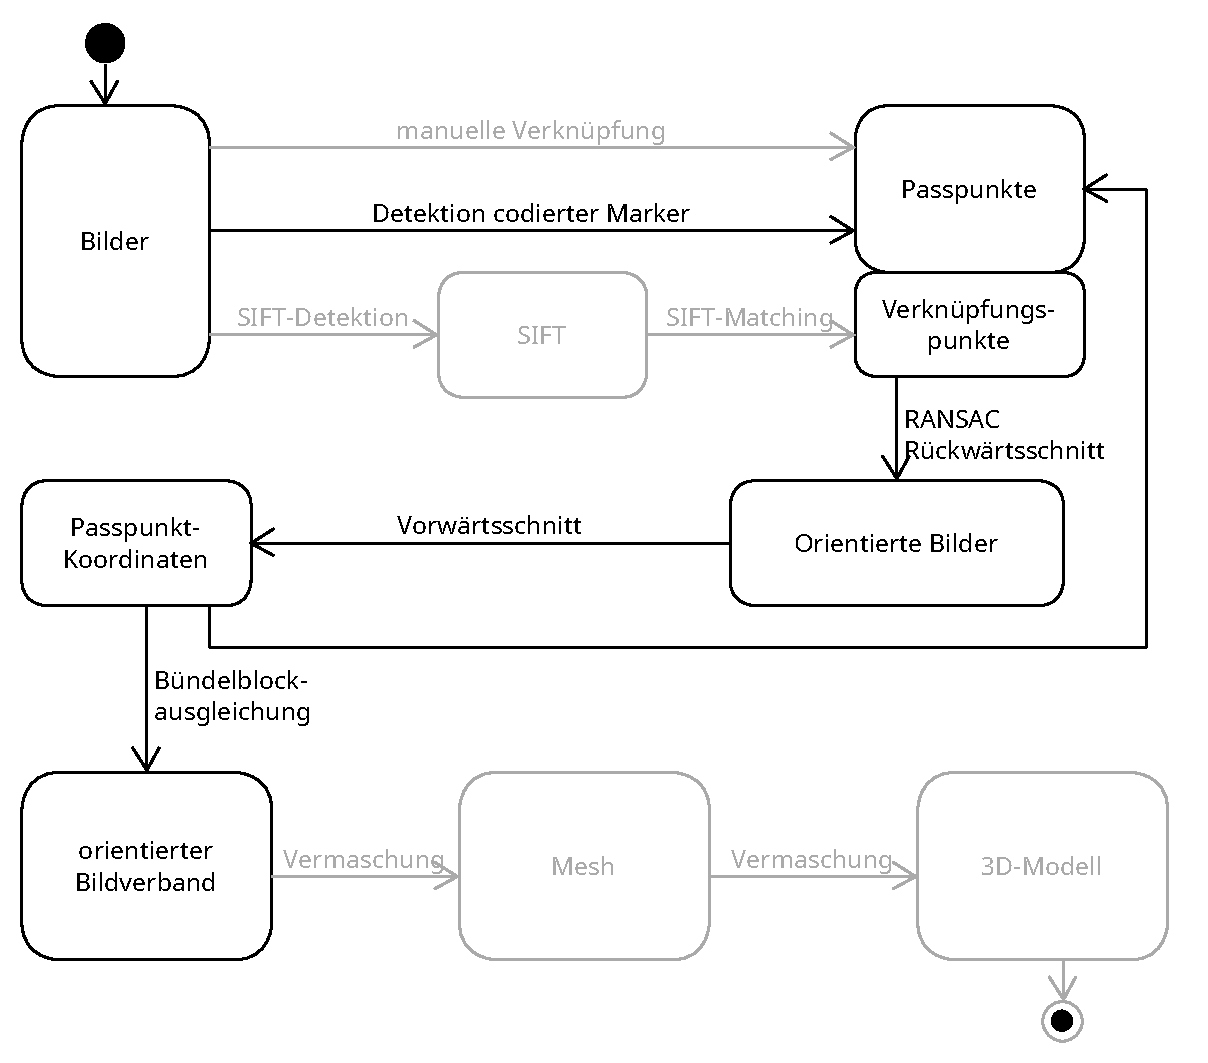
\includegraphics[width=0.9\textwidth]{./img/uml/uml_ablauf.pdf}
    \caption{Ablauf der Bildverknüpfung mittels \acrfull{SfM}, nach \citealt[S. 492]{luhmann}}
    \label{img:ablauf}
\end{figure}

Zunächst werden die Bilder aufgenommen (siehe \autoref{s:bilder}). Hierbei ist wichtig, dass sich die Bildinhalte überlappen. Die Bilder werden dann verknüpft, indem identische Punkte in den Bildern identifiziert werden  (siehe \autoref{s:verknuepfung}).
Aus den identifizierten Punkten werden dann die Positionen und Ausrichtung der Kameras und Verknüpfungspunkte in einem lokalen Koordinatensystem ohne bekannten Maßstab berechnet. Die so erzeugten Daten werden anschließend in einer Bündelblockausgleichung gemeinsam optimiert (siehe \autoref{s:buendelblock}). Durch die Nutzung von bekannten Größen, beispielsweise kalibrierten Maßstäben, kann dieses System transformiert werden.

\section{Abbildung}
\label{s:abbildung}
Grundlage der Photogrammetrie ist die Abbildungsgleichung. Diese beschreibt die Abbildung eines Punktes im Raum auf dem Sensor beziehungsweise dem Film. Umgekehrt kann mit ihrer Hilfe aus der Position eines Punktes in einem Bild, ähnlich einer Messung mit einem Theodolit, die Richtung des Punktes in Relation zu der Kamera bestimmt werden. Die Abbildungsgleichung ist abhängig von der inneren und äußeren Orientierung der Kamera. Die \gls{innereOrientierung} beschreibt die Abbildungseigenschaften der Kamera, die \gls{aeussereOrientierung} die Position und Ausrichtung der Kamera. Im Folgenden wird zuerst auf die innere und \gls{aeussereOrientierung} eingegangen, bevor die Abbildungsgleichung selbst vorgestellt wird.

\subsection{Innere Orientierung}
\label{s:innereorientierung}
Die \gls{innereOrientierung} beschreibt die Abbildungseigenschaften der Kamera auf mathematische Weise. Parameter sind hierbei die Lage des \Gls{Bildhauptpunkt}es, die Kamerakonstante sowie die Parameter, die die \Gls{Verzeichnung} beschreiben. \citep[vgl.][S. 179f]{luhmann}

Normalerweise wird die Kamera hierbei vereinfacht als Lochkamera unter Verwendung der Zentralperspektive betrachtet (siehe \autoref{img:optische_achse}). Als Projektionszentrum $O'$ wird hierbei der Punkt beschrieben, durch den alle Bildstrahlen geradlinig laufen. Sein Lot auf dem Sensor wird als \Gls{Bildhauptpunkt} $H'$ bezeichnet und beispielsweise durch seine Lage in Pixeln oder Mikrometern beschrieben. Durch eine schiefe optische Achse kann dieser vom Mittelpunkt des Sensors abweichen. Die \Gls{Kamerakonstante} $c$ beschreibt idealisiert den Abstand des Projektionszentrums zum Sensor. \citep[vgl.][S. 177]{luhmann}

\begin{figure}[htbp]
    \centering
    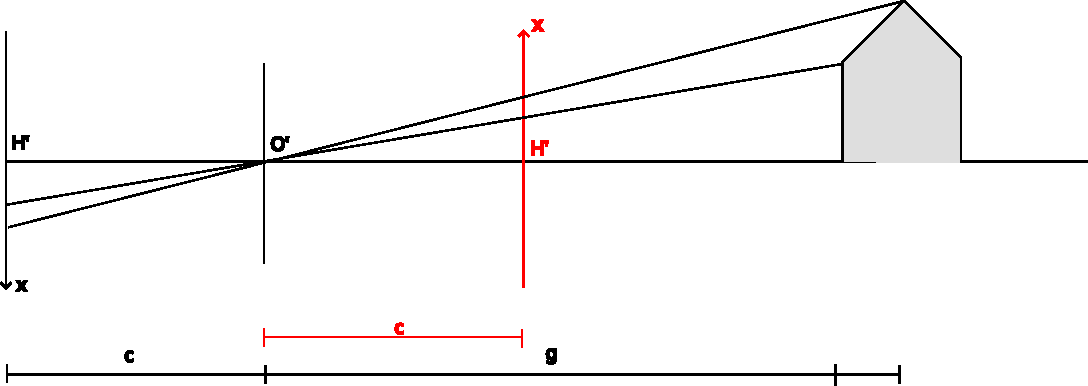
\includegraphics[width=0.8\textwidth]{./img/2_grundlagen/optischeAchse.pdf}
    \caption{Abbildung des Lochkamera-Modells mit Spiegelung am Projektionszentrum (rot), nach \citet[S. 154]{hartley}, Beschriftung nach \citet[S. 177]{luhmann}}
    \label{img:optische_achse}
\end{figure}

Als \Gls{Verzeichnung} wird die Abweichung der Abbildung von der idealen Lochkamera bezeichnet. Diese kann durch die Nutzung von Linsen oder durch die Bauweise der Kamera entstehen. Die \Gls{Verzeichnung} wird in radialer und tangentialer \Gls{Verzeichnung} unterschieden. Die radiale \Gls{Verzeichnung} beschreibt die Verschiebung der Bildpunkte zur Bildmitte hin. Dieser Punkt wird Symmetriepunkt genannt und muss nicht zwangsläufig mit dem Bildhauptpunkt zusammenfallen, für die Korrekturen wird dieses jedoch üblicherweise so angenommen. Die tangentiale \Gls{Verzeichnung} beschreibt die Verschiebung quer zur radialen Richtung. Am wichtigsten ist hierbei die radial-symmetrische \Gls{Verzeichnung}, da diese die größte Auswirkung hat. Sie entsteht durch den nicht symmetrischen Aufbau des Objektives vor und hinter der Blende. Die radial-asymmetrische und die tangentiale \Gls{Verzeichnung}en entstehen hauptsächlich aus einer Dezentrierung und Schiefstellung der Linsen zur optischen Achse. \citep[vgl.][S. 178]{luhmann}

Jede Einstellung der Kameraoptik verändert die \gls{innereOrientierung} und jede Kamera, selbst in derselben Modellreihe, unterscheidet sich in ihren Parametern. Änderungen können sich beispielsweise durch Umfokussierung oder die Nutzung eines optischen Zoom ergeben, als auch durch einen mechanisch instabilen Aufbau der Kameras oder Erwärmung und der damit verbundenen Ausdehnung. Daher sollten die Bilder normalerweise möglichst mit nur einer Kamera mit festen Einstellungen (Brennweite, Fokus, Blende, Objektiv) aufgenommen werden. Änderungen der Empfindlichkeit (ISO-Zahl) oder Belichtungszeit sind unproblematisch für die \gls{innereOrientierung}, da hierbei die Abbildungseigenschaften der Kamera nicht verändert werden. \citep[vgl.][S. 176]{luhmann}

Die genaue Bestimmung der inneren Orientierung, auch Kalibrierung genannt, kann wäh\-rend der Messung beispielsweise als Parameter in der Bündel\-block\-ausgleichung erfolgen. Je nach Anzahl der Kameras und Stabilität der inneren Orientierung sind hier verschiedene Varianten möglich. Bei stabilen Kameras wird ein Parameter-Satz pro Kamera für eine ganze Messreihe ausgeglichen, bei instabilen Kameras kann die Kalibrierung jedes einzelnen Bildes notwendig werden. \citep[vgl.][S. 181f]{luhmann}

\subsection{Äußere Orientierung}
\label{s:aeussereorientierung}
Die \gls{aeussereOrientierung} beschreibt die Lage der Kamera im Raum und ihre Ausrichtung. Sie wird durch die Position des Projektionszentrums und die Richtung der optischen Achse beschrieben. Die Position wird hierbei durch 3D-Koordinaten beschrieben, in der Nahbereichsphotogrammetrie oft in einem lokalen System. Die Richtung der optischen Achse wird mit der Rotation der Kamera zu diesem Koordinatensystem beschrieben, beispielsweise durch eine Rotationsmatrix, eulersche Winkel oder Quaternionen. Durch die Nutzung von Passpunkten oder bekannten Koordinaten der Kamera kann die \gls{aeussereOrientierung} bestimmt werden. \citep[vgl.][S. 273ff]{luhmann}

Die Darstellung der Rotation der Kamera als Quaternionen hat den Vorteil, dass diese dann mit nur vier Parametern in eine Bündelblockausgleichung eingeht. Bei der Nutzung der Rotationsmatrix hätte man hier neun bzw. acht unabhängige Parameter. Die Nutzung von eulerschen Winkeln hat den Nachteil, dass hier ein sogenannter Gimbal-Lock auftreten kann, bei dem zwei Achsen zusammenfallen und die Rotation nicht mehr eindeutig bestimmt werden kann. \citep[vgl.][S. 63]{luhmann}

\subsection{Abbildungsgleichung}
\label{ss:abbildungsgleichung}
Die Abbildung eines Punktes auf einem Bild wird durch die Abbildungsgleichung beschrieben. Hierfür gibt es verschiedene Schreibweisen. In der Matrizenrechnung besteht diese aus der Multiplikation der homogenen Punktkoordinaten $X$ mit der Projektionsmatrix $P$ (\autoref{eq:abbildungsgleichung}). $P$ ergibt sich aus der Kalibrier- oder Kameramatrix $K$, der Rotation $R$ und dem Vektor zum Projektionszentrum $X_0$ (\autoref{eq:pkr}). Die Kalibriermatrix wiederum besteht aus der \Gls{Kamerakonstante} und der Lage des \Gls{Bildhauptpunkt}es (\autoref{eq:k}, nach \citealp[S. 244]{hartley} und \citealp[S. 290]{luhmann}).

Die \gls{aeussereOrientierung} ist durch die Matrix $[R|X_0]$ beschrieben (\autoref{eq:r}). Diese besteht aus der Rotationsmatrix $R$ und dem Vektor zum Projektionszentrum $X_0$. Die Rotationsmatrix beschreibt die Ausrichtung der Kamera im Raum, das Projektionszentrum beschreibt die Position der Kamera bzw. des Projektionszentrums im Raum.

\begin{align*}
    \nlabel{eq:abbildungsgleichung}
    x'      & = P \cdot X       \\
    \nlabel{eq:pkr}
    P       & = K \cdot [R|X_0] \\
    \nlabel{eq:k}
    K       & =
    \begin{bmatrix}
        c_x & 0   & x'_0 \\
        0   & c_y & y'_0 \\
        0   & 0   & 1    \\
    \end{bmatrix}            \\
    \nlabel{eq:r}
    [R|X_0] & =
    \begin{bmatrix}
        r_{11} & r_{21} & r_{31} & X_0 \\
        r_{12} & r_{22} & r_{32} & Y_0 \\
        r_{13} & r_{23} & r_{33} & Z_0 \\
    \end{bmatrix}
\end{align*}
\begin{conditions}
    x' & Bildkoordinate \\
    P  & Projektionsmatrix \\
    X  & Homogene Punktkoordinaten \\
    K  & Kalibrier- oder Kameramatrix \\
    R  & Rotationsmatrix \\
    X_0 & Vektor zum Projektionszentrum \\
    c_x, c_y & \Gls{Kamerakonstante} in x- und y-Richtung \\
    x'_0, y'_0 & Lage des \Gls{Bildhauptpunkt}es in x- und y-Richtung \\
    r_{mn} & Parameter der Rotationsmatrix \\
\end{conditions}

% Um die Beziehung zwischen zwei Bildern aufzustellen, kann man diese Abbildungsgleichung nutzen. Da es hier nur um die Beziehung zwischen zwei Bildern geht, kann die Rotation und Translation des ersten Bildes auf 0 gesetzt werden ($R$ ist dann eine 3x3-Einheitsmatrix und $X_0$ ein Nullvektor). $X_0$ des zweiten Bildes wird zur Translation zwischen den beiden Bildern. \citep[vgl.][S. 330]{luhmann}

Grundlage dieser Formel ist das Lochkamera-Modell (siehe \autoref{img:optische_achse}). Dabei wird rechnerisch das Bild an dem Projektionszentrum in den Objektraum gespiegelt (rot im Bild). Dadurch kann mit einem aufrechten Bild gerechnet werden.

Als weitere Parameter spielt die \Gls{Verzeichnung} eine Rolle. Diese können in die Abbildungsgleichung integriert werden, in dem $x'$ durch $\Delta x'$ korrigiert wird. \citep[vgl.][S. 277]{luhmann}

\begin{align*}
    \nlabel{abbildungsgleichung_verzeichnung}
    x'        & = P \cdot X + \Delta x'                 \\
    \Delta x' & = \Delta x_{rad} + \Delta x_{tan} + ...
\end{align*}
\begin{conditions}
    \Delta x' & \Gls{Verzeichnung} \\
    \Delta x_{rad} & radial-symmetrische \Gls{Verzeichnung} \\
    \Delta x_{tan} & tangentiale \Gls{Verzeichnung} \\
\end{conditions}

Die \Gls{Verzeichnung} wird meist mit den Parametern $k_1$ bis $k_4$ für die radial-symmetrische \Gls{Verzeichnung} und $p_1$ und $p_2$ für die tangentiale \Gls{Verzeichnung} bezeichnet. Die Faktoren stellen dabei die Parameter einer Taylor-Reihe dar. Sie basieren auf dem Kameramodell von \citet[S. 859]{brown1971} und denen von ihm vorgestellten Formeln (\autoref{eq:brown_rad} und \ref{eq:brown_tan}).

\begin{align*}
    \nlabel{eq:brown_rad}
    \Delta x_{rad} & = k_1 \, r^2 + k_2 \, r^4 + k_3 \, r^6 + k_4 \, r^8                  \\
    \Delta y_{rad} & = k_1 \, r^2 + k_2 \, r^4 + k_3 \, r^6 + k_4 \, r^8                  \\
    \nlabel{eq:brown_tan}
    \Delta x_{tan} & = p_1 \, (r^2 + 2 \,\bar{x}^2) + 2\, p_2  \,  \bar{x}  \, \bar{y}    \\
    \Delta y_{tan} & = 2  \, p_1 \,  \bar{x}  \, \bar{y} +  p_2 \, (r^2 + 2 \, \bar{y}^2) \\
    r              & = \sqrt{\bar{x}^2 + \bar{y}^2}                                       \\
    \bar{x}        & = x' - x'_0                                                          \\
    \bar{y}        & = y' - y'_0
\end{align*}
\begin{conditions}
    r                   & Abstand des Punktes zum \Gls{Bildhauptpunkt}          \\
    x', y'              & Bildkoordinaten                                      \\
    \bar{x}, \bar{y}    & Abstand von Bildhauptpunkt in x- bzw. y-Richtung      \\
    k_1, k_2, k_3, k_4  & Radial-symmetrische \Gls{Verzeichnung}sparameter                  \\
    p_1, p_2            & Tangentiale \Gls{Verzeichnung}sparameter              \\
\end{conditions}

Diese Parameter werden so beispielsweise auch in Photogrammetrie- und Computer-Vision-Software wie Agisoft Metashape, OpenDroneMap und OpenCV genutzt.

\section{Bilder}
\label{s:bilder}

Die Berechnung der Position eines Objektes im Bild ist nur möglich, sofern der Punkt in mindestens einem weiteren Bild abgebildet ist. Die Genauigkeit der Berechnung ist vom Schnittwinkel dieser beiden Strahlen abhängig. Um möglichst gute Grundlagen zur Ver\-fügung zu haben und die innere und \gls{aeussereOrientierung} möglichst gut berechnen zu können, müssen diese Bilder einige Bedingungen erfüllen - auf diese wird hier eingegangen.

\subsection{Überlappung und Bildinhalte}
Da die Bilder durch identische Punkte verbunden werden, müssen sich die Bildinhalte überlappen und gemeinsame Punkte in den Bildern identifiziert werden. Die au\-to\-ma\-tische Detektion von identischen Punkten ist auf verschiedene Weisen möglich: Entweder durch die Nutzung von codierten und uncodierten Passpunkten oder über eine Merk\-mals\-ex\-trak\-tion. Für letzteres muss die Oberfläche genügend Textur bzw. Struktur aufweisen. Detailliert wird in \autoref{s:verknuepfung} hierauf eingegangen. \citep[vgl.][S. 478]{luhmann}

\subsection{Position und Ausrichtung der Kamera}
Damit die Schnitte der Bildstrahlen optimal sind und die Berechnung der Tiefeninformationen möglichst genau ist, müssen die Kameras möglichst gleichmäßig um das Objekt verteilt sein.
Bilder, die vom gleichen Standpunkt aufgenommen wurden, sind oft nur ungenau verknüpfbar. Daher empfiehlt es sich, Bilder aus verschiedensten Richtungen zu machen, also bei der manuellen Photographie um das Objekt herumzugehen und eine Mehrbildaufnahme im Rundum-Verband zu erzeugen. \citep[vgl.][S. 170]{luhmann}

Entsprechend müssen die Kameras gleichmäßig um das Objekt verteilt positioniert werden und dabei auch an die Form des Objektes wie Einschnitte anpassbar sein.

\subsection{Belichtung}
Um identische Punkte in den Bildern identifizieren zu können, müssen die Bilder eine gleichmäßige Beleuchtung aufweisen. Hierfür sollte es vermieden werden, dass Schatten auf das Objekt fallen. Eine gleichmäßige Beleuchtung kann durch die Nutzung von mehreren Lichtquellen erreicht werden. Auch sollte keine Blendwirkung entstehen, die durch direkte Sonneneinstrahlung oder Reflexionen entstehen kann. Die Belichtung der einzelnen Bilder sollte möglichst identisch sein, damit später auch eine zusammenhängende Texturierung möglich ist.
Da die Objekte und die Kameras sich während der Aufnahme nicht bewegen, kann die Belichtungszeit verlängert werden, um Rauschen durch eine zu hohe Sensorempfindlichkeit zu vermeiden und so die Bildqualität zu erhöhen.


\subsection{Fokussierung und Schärfentiefe}
\label{s:schaerfe}
Um genaue Punktwolken erzeugen zu können, muss das Objekt scharf abgebildet werden. Die Kameras müssen dafür entsprechend fokussiert sein. Jedoch wird durch die Fokussierung auch die \gls{innereOrientierung} verändert. Normalerweise wird daher auf eine Umfokussierung verzichtet und mittels der Blende (kleine Blendenöffnung) die Schärfentiefe erhöht, sodass ein großer Bereich scharf abgebildet wird. Dieses ist aber bei vielen einfachen Kameras wie dem verwendeten Raspberry Pi Camera Module 3 nicht möglich.

Der Schärfebereich ergibt sich aus der Größe des tolerierbaren Unschärfekreises auf dem Sensor. Bei digitalen Kameras wird dieser durch die Pixelgröße bestimmt. Nach \citet[S. 148f]{luhmann} berechnet sich die Schärfentiefe nach folgender Formel:

\begin{align*}
    \nlabel{eq:schaerfebereich}
    t   & = a_h - a_v            \\
    a_v & = \frac{a}{1+K}        \\
    a_h & = \frac{a}{1-K}        \\
    K   & = \frac{k(a-f)u'}{f^2}
\end{align*}
\begin{conditions}
    t   & Länge des Schärfebereichs \\
    a_v, a_h & vordere bzw. hintere Grenze der Schärfentiefe\\
    a   & fokussierte Dingweite\\
    k   & Blendenzahl\\
    f   & Brennweite
\end{conditions}

Die Schärfentiefe des Raspberry Pi Camera Module 3 ist in \autoref{img:sschaerfentiefe_plot} für einen Unschärfekreis von drei Pixeln dargestellt (Plot der \autoref{eq:schaerfebereich}). Es zeigt sich, dass die Schärfentiefe im  verwendeten Makrobereich relativ klein ist. Problematisch ist dies vor allem bei größeren Objekten, die hierdurch näher an die Kameras rücken, aber durch ihre Größe eine größere Schärfentiefe benötigen. Ein Lösungsansatz durch Kombination mehrerer Aufnahmen wird in \autoref{sec:fokusstacking} untersucht.

\begin{figure}[htbp]
    \centering
    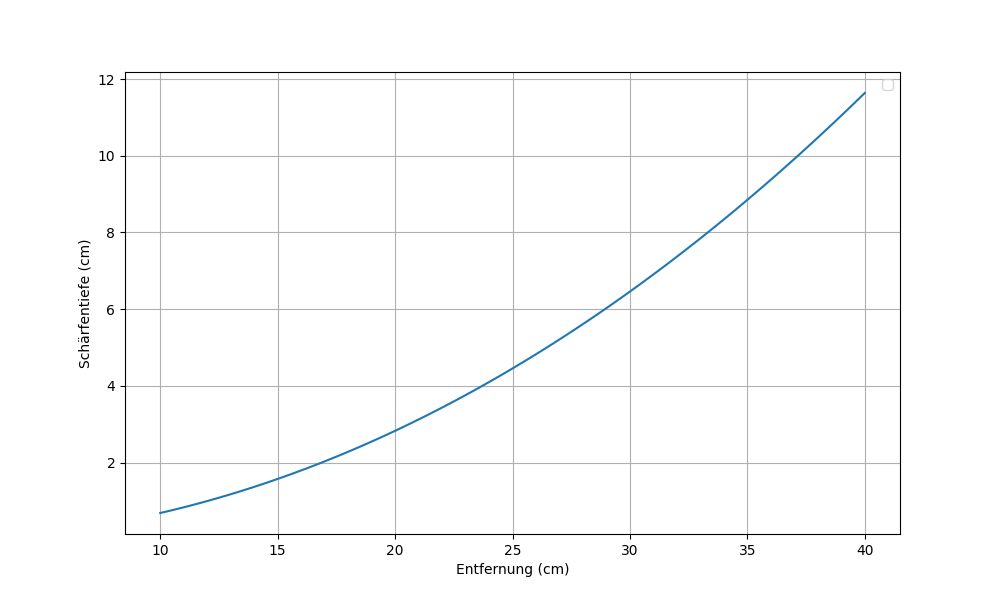
\includegraphics[width=0.9\textwidth]{./img/2_grundlagen/schaerfentiefe_plot.png}
    \caption{Schärfentiefe in Abhängigkeit von der fokussierten Entfernung}
    \label{img:sschaerfentiefe_plot}
\end{figure}


\section{Skalierung/Maßstab}
\label{sec:massstab}
Die Skalierung eines rein photogrammetrisch bestimmten 3D-Modelles ist nicht bekannt, da die Berechnungen nur auf Richtungen ohne Längenangaben basieren - es ist im mathematischen Sinne \gls{aehnlich} dem realen Körper. Daher werden Referenzen in Form einer bekannten Länge benötigt, um die Skalierung zu bestimmen. Alternativ können auch Passpunkte (siehe \autoref{s:verknuepfung}) mit bekannten Koordinaten verwendet werden oder im Falle von Mehrkamerasystemen bekannte \gls{aeussereOrientierung}en der Kameras. \citep[vgl.][S. 546]{luhmann}


\section{Verknüpfungs- und Passpunkte}
\label{s:verknuepfung}
Um die einzelnen Bilder verknüpfen zu können, werden identische Punkte zwischen zwei oder mehr Bildern benötigt. Diese können klassisch manuell erfasst werden, jedoch ist dieses schon bei kleineren Projekten sehr zeitaufwändig. Daher wird meist die Möglichkeit genutzt, au\-to\-ma\-tisch Verknüpfungspunkte zu erzeugen. Hierfür gibt es unterschiedliche Methoden, die im Folgenden vorgestellt werden.


\subsection{Zielmarker}
Es gibt verschiedenste Formen von Markern, die au\-to\-ma\-tisch erfasst werden können. Grob unterschieden werden kann in codierte und nicht codierte Zielmarker. Beispiele für nicht codierte sind beispielsweise einfache kreisförmige Klebepunkte oder Marker, die aus Linien bestehen und ihren Mittelpunkt durch dessen Schnitt definieren.
Vorteilhaft ist jedoch die Verwendung von codierten Zielmarken. Hier können die Punkte direkt zugeordnet werden, sodass keine weitere Filterung und Berechnung zur Zuordnung notwendig ist. \citep[vgl.][S.535ff]{luhmann}

\subsubsection{Zielmarken nach Schneider}
Eine Form der codierten Zielmarken sind die Marker nach Schneider. Diese bestehen aus mehreren konzentrischen Kreisen (siehe \autoref{img:schneider}) und werden entsprechend als \Gls{CCCT} bezeichnet \citep[vgl.][]{ccct}. Die Mitte des Markers wird durch den gemeinsamen Mittelpunkt der Kreise definiert \citep[vgl.][]{schneider}. Vorteilhaft ist, dass die Marker auch bei unscharfen Bildern erkannt werden können und ihr Zentrum manuell identifiziert werden kann, beispielsweise zum Aufmaß mit einem Tachymeter. Sie haben sich daher als Standardmarker in der Photogrammetrie etabliert und werden beispielsweise von Agisoft Metashape verwendet.


\begin{figure}[htbp]
    \centering
    \begin{subfigure}{0.45\textwidth}
        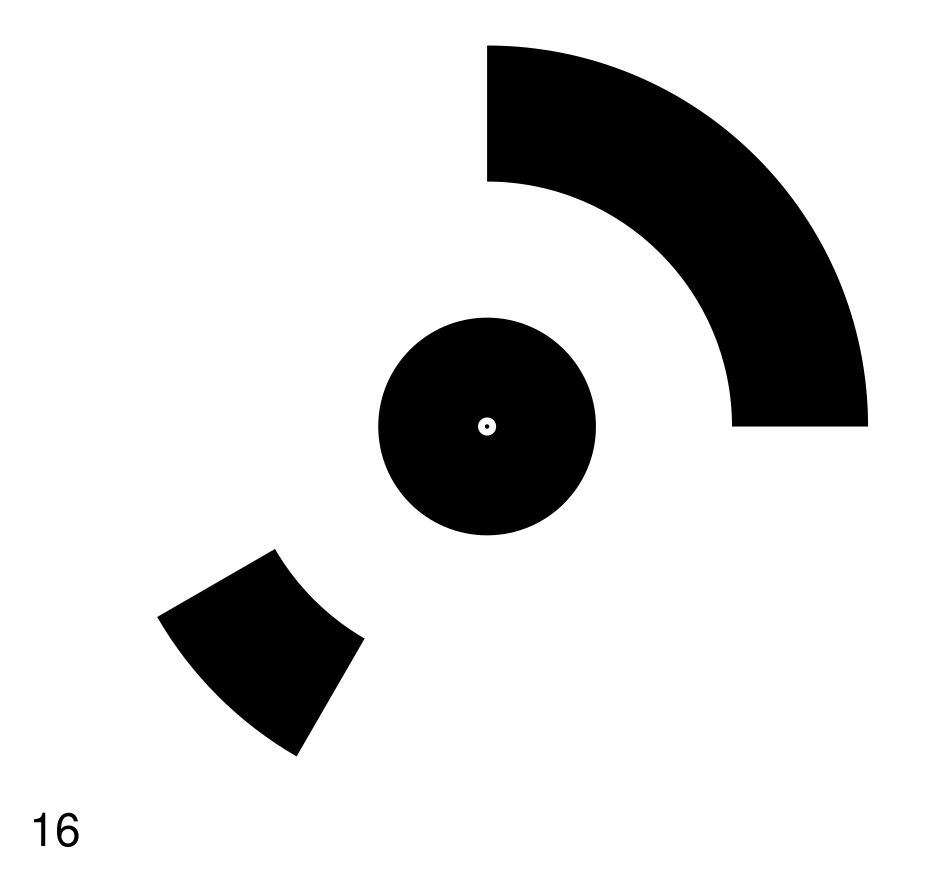
\includegraphics[width=0.98\linewidth]{img/2_grundlagen/schneider.png}
        \centering
        \caption{\acrshort{CCCT} nach \\ \citet{schneider},\\aus Agisoft Metashape}
        \label{img:schneider}
    \end{subfigure}
    \begin{subfigure}{0.45\textwidth}
        
\includegraphics[width=0.98\linewidth]{img/2_grundlagen/aruco.png}
        \centering
        \caption{ArUco-Marker,\\generiert mit \citet{opencv}\\}
        \label{img:aruco}
    \end{subfigure}
    \caption{Codierte Passpunkte}
\end{figure}

\subsubsection{ArUco-Marker}
Eine andere Variante der codierten Verknüpfungspunkte sind die sogenannten ArUco-Marker (siehe \autoref{img:aruco}). Diese werden häufig für die Orientierung bei Augmented-Reality-An\-wend\-ungen genutzt. Jede Ecke kann hierbei au\-to\-ma\-tisch im Subpixelbereich identifiziert werden, sodass ein erkannter Marker vier Verknüpfungspunkte liefern kann. Wenn deren (lokale) Koordinaten und die \gls{innereOrientierung} bekannt sind, kann mit nur einem Marker die \gls{aeussereOrientierung} bestimmt werden. \citep[vgl.][S. 545]{luhmann}

Nachteilig zeigte sich in den Untersuchungen des Fokus (siehe \autoref{sec:fokus}), dass die Ecken nicht eindeutig identifiziert werden können, wenn die Aufnahme unscharf ist. Durch ihre Verwendung in Augmented-Reality-Anwendungen sind auch viele kostenfreie Bibliotheken für ihre Erkennung verfügbar, sodass beispielsweise \citet{opencv} ArUco-Marker identifizieren kann.


\subsection{Merkmalsextraktion}
\label{ss:sift}
Auch ohne das Anbringen von Markern können Verknüpfungspunkte erzeugt werden. Hierfür wird Merk\-mals\-ex\-trak\-tion verwendet, beispielsweise \Gls{SIFT}, welches hier stellvertretend kurz vorgestellt wird. Es liefert Verknüpfungspunkte aus Mustern auf den photographierten Oberflächen. Es ist meist nicht notwendig, explizit Marker an dem aufzunehmenden Objekt anzubringen, sofern seine Oberfläche nicht strukturlos ist (glatte weiße Wände etc.).

Zur Erkennung von Merkmalen setzt \gls{SIFT} auf die Detektion von Kanten. Diese werden in verschiedenen Stufen einer Bildpyramide erkannt und ihre Extrema berechnet. Sie werden anschließend weiter ausgedünnt, beispielsweise über den Kontrast. Sofern ein möglicher Marker identifiziert wurde, wird eine Beschreibung erzeugt. Diese erfolgt  durch Analyse der Helligkeitsabweichungen zu den Nachbar-Pixeln und wird an der stärksten Abweichung ausgerichtet. Hierdurch wird die Beschreibung dann richtungsunabhängig. Mit den Beschreibungen kann dann die Übereinstimmung von zwei Markern in zwei Bildern identifiziert werden, auch wenn diese zueinander gekippt oder gedreht sind.
\citep[vgl.][S. 484f]{luhmann}

\section{Verknüpfung von Bildern}
\label{s:photogramm}
Durch die beschriebenen Verfahren und die hieraus entstandenen Verknüpfungs\-punkte können die Bilder miteinander verknüpft werden. Da die Kamerapositionen am Rahmen veränderlich sind und die Montage auch keine ausreichend genaue Fixierung garantiert, können die bekannten Positionen aus vorherigen Messungen maximal als Näherungswerte genutzt werden. Die genaue Bestimmung der Position und Ausrichtung - die \gls{aeussereOrientierung} - muss daher mindestens für die verschobenen oder gedrehten Kameras neu berechnet werden. Gleiches gilt für neue Verknüpfungspunkte, für die noch keine Koordinate bekannt ist. Die verwendeten Methoden, die so zur Verknüpfung der Bilder beitragen, werden im Folgenden vorgestellt: der Rückwärts-, der Vorwärtsschnitt und die relative Orientierung.

\subsection{Rückwärtsschnitt}
Sofern Koordinaten von Passpunkten bekannt sind, können die Positionen und Ausrichtungen der Kameras berechnet werden. Hierfür wird der sogenannte Rückwärtsschnitt genutzt. Die Berechnung erfolgt auf Basis der Abbildungsgleichung, die die Position eines Punktes in einem Bild in Beziehung zur Kamera setzt. Für die Berechnung selbst gibt es verschiedene Methoden. Verwendet wurde hier der von OpenCV genutzte Ansatz von \citet{Lepetit2008} in Kombination mit einem RANSAC-Ansatz.

Durch die Nutzung des RANSAC-Ansatzes können veränderte Passpunkte identifiziert und als Ausreißer markiert werden. Hierzu werden mehrere Stichproben der Punkte gewählt, die Berechnung durchgeführt und die Lösung gewählt, zu denen die meisten Punkte passen. \citep[vgl.][S. 134]{luhmann}

\autoref{img:rueckwaertsschnitt} zeigt die geometrischen Grundlagen des Rückwärtsschnittes. Es müssen mindestens 3 Passpunkte ($P_1 - - P_3$) mit Koordinaten bekannt und im Bild sichtbar sein. Außerdem muss die \gls{innereOrientierung} bei Verwendung von nur drei Passpunkten bekannt sein. Die Position der Punkte $P'_1 - - P'_3$ wird dann bestimmt und ergibt im Beispiel 6 Koordinatenkomponenten (jeweils $x'$ und $y'$). Durch Berechnungen -- auf die hier nicht weiter eingegangen und auf entsprechende Literatur verwiesen wird -- kann dann die Position (drei Parameter) und Ausrichtung (drei Parameter) der Kamera bestimmt werden. \citep[vgl.][S. 284]{luhmann}

\begin{figure}[htbp]
    \centering
    \begin{subfigure}{0.45\textwidth}
        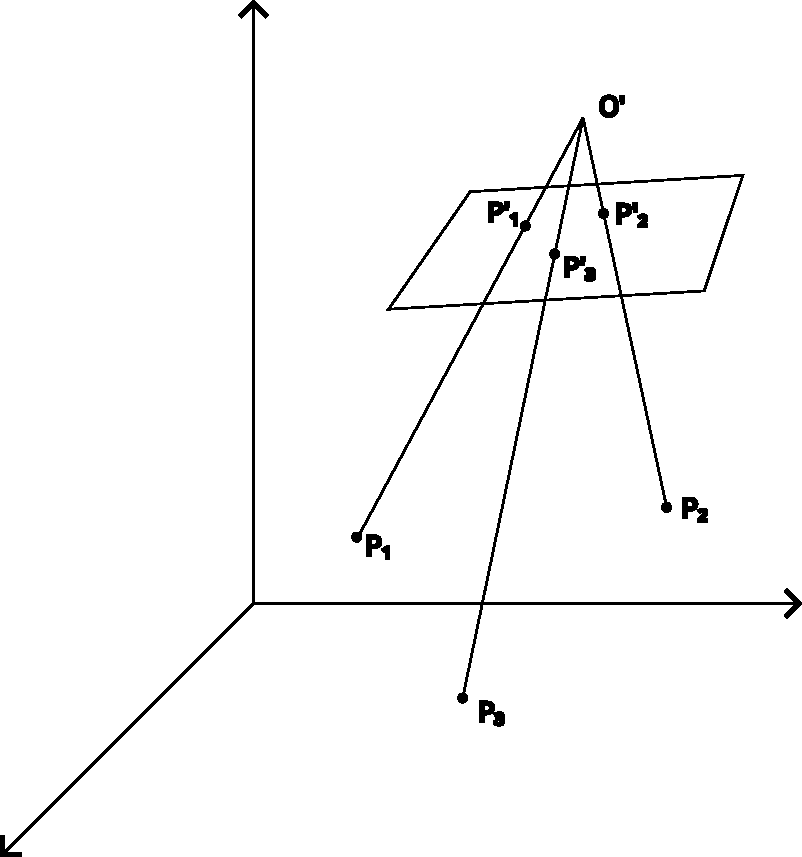
\includegraphics[width=0.9\linewidth]{img/2_grundlagen/rueckwaertsschnitt.pdf}
        \centering
        \caption{Rückwärtsschnitt, nach \\ \citealt[S. 284]{luhmann}}
        \label{img:rueckwaertsschnitt}
    \end{subfigure}
    \begin{subfigure}{0.45\textwidth}
        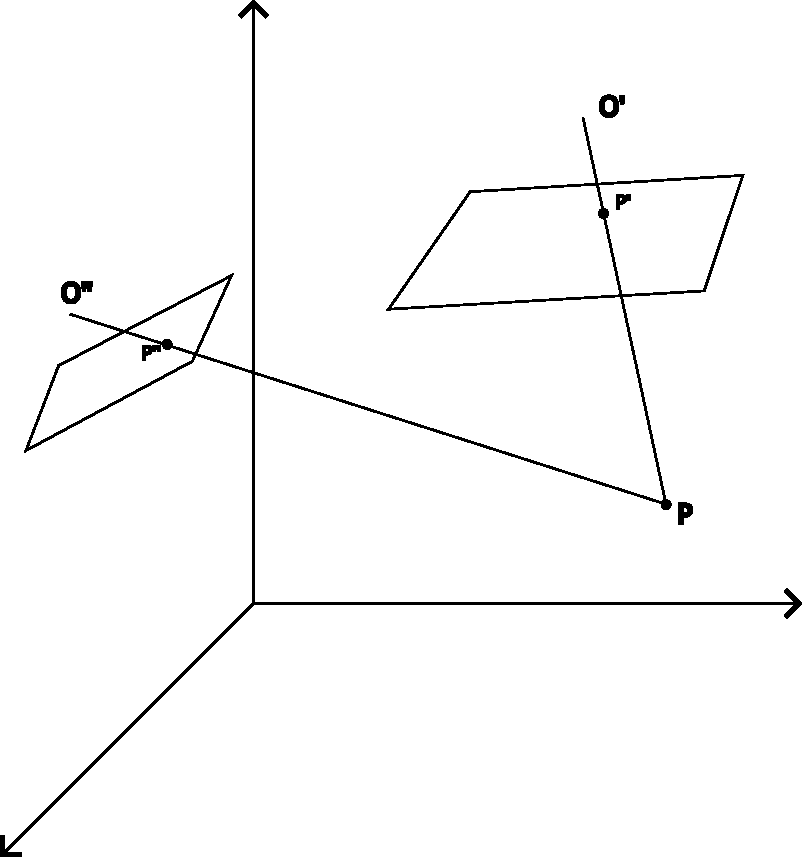
\includegraphics[width=0.9\linewidth]{img/2_grundlagen/vorwaertsschnitt.pdf}
        \centering
        \caption{Vorwärtsschnitt, nach \\ \citealt[S. 339]{luhmann}}
        \label{img:vorwaertsschnitt}
    \end{subfigure}
    \caption{Geometrische Grundlagen des Rückwärts- und Vorwärtsschnittes}
\end{figure}

\subsection{Vorwärtsschnitt}
Um wiederum aus einem Stereopaar mit bekannter innerer und äußerer Orientierung Punktkoordinaten zu berechnen, wird der Vorwärtsschnitt genutzt. \autoref{img:vorwaertsschnitt} zeigt die geometrischen Grundlagen des Vorwärtsschnitts. Es werden die Bildkoordinaten der Punkte $P_1$ und $P_2$ benötigt, die im Bild sichtbar sind. Die Position des Punktes $P$ wird dann berechnet. Wie bereits in \autoref{s:abbildung} erwähnt, kann jeder Punkt im Bild durch die \gls{innereOrientierung} als Horizontal- und Vertikalrichtungsmessung interpretiert werden. Durch die \gls{aeussereOrientierung} kann diese dann ins übergeordnete System überführt werden. Hieraus ergibt sich dann zur Berechnung der Position $P$ ein räumlicher Schnitt zweier (windschiefer) Geraden \citep[vgl.][S. 95]{luhmann}.

Mit dem Vorwärts\-schnitt können neben markierten Verknüpfungspunkten auch die Neupunkte, die mittels SIFT oder ähnlicher Bild\-erkennungs\-algorithmen erkannt wurden, berechnet werden. Dadurch kann eine dünne Punktwolke erzeugt werden, welche dann bei der Bündelblockausgleichung (siehe \autoref{s:buendelblock}) genutzt werden kann. Da die Berechnung bereits bei Bildkoordinaten aus zwei Bildern überbestimmt ist und oft Punkte in mehr Bildern abgebildet sind, bietet sich die Nutzung einer Ausgleichung auch schon bei der Bestimmung an. \citep[vgl.][S. 385]{luhmann}

\subsection{Relative Orientierung}
\label{ss:relative_orientierung}
Wenn keine Passpunkte vorhanden sind und durch zum Beispiel ArUco-Marker keine lokalen Passpunkt-Koordinaten erzeugt werden können, kann die Bildorientierung auch in einem lokalen System erfolgen. Hierbei wird die relative Orientierung der Bilder zueinander bestimmt. Eines der Bilder wird als Ursprung des Systems festgelegt (Projektionszentrum in $(0,0,0)$ und die optische Achse in $z$-Richtung). Die Position und Ausrichtung des zweiten Bildes wird dann relativ zu diesem bestimmt. \citep[vgl.][S. 316]{luhmann}

Die klassische Variante der relativen Orientierung ist die Bestimmung der Essenziellen Matrix, welche identische Punkte in einem Bild mit denen in einem anderen Bild in Beziehung setzt. Diese kann aus der inneren Orientierung und der Fundamentalmatrix berechnet werden, welche wiederum aus den Bildkoordinaten von mindestens 8 Verknüpfungspunkten berechnet werden kann. \citep[vgl.][S. 328ff]{luhmann}

Mittels Einzelwertzerlegung kann dann aus der Essenziellen Matrix die Rotation und Translation des zweiten Bildes bestimmt werden. \citep[vgl.][S. 275]{hartley}

Alternativ kann mit der Homographie die relative Orientierung über eine Ebene, die in beiden Bildern abgebildet wird, bestimmt werden. Dieser Fall tritt beispielsweise bei der Verwendung von flächenhaften Kalibriermustern auf. Die Homographie beschreibt die Abbildung einer Ebene auf eine andere Ebene. Sie wird durch eine 3x3-Matrix beschrieben, die die Transformation der Punkte beschreibt. Für die Bestimmung werden nur 4 Verknüpfungspunkte benötigt, die in beiden Bildern sichtbar sind und auf einer Ebene liegen. Die \gls{innereOrientierung} der Kamera wird hierbei nicht benötigt. \citep[vgl.][S. 33ff]{hartley}.

Aus der Homographie kann zusammen mit der inneren Orientierung die Rotation und Translation des zweiten Bildes bestimmt werden.
\citep[vgl.][S. 74]{homography_decomposition}


\begin{comment}
Die Koordinaten der Passpunkt-Ausreißer aus der Berechnung der Kamerapositionen werden anschließend neu berechnet. Hierfür wird der Vorwärtsschnitt genutzt. Auch hier wird OpenCV zur Berechnung genutzt. Die Berechnung der Passpunkte erfolgt für jedes Bildpaar einzeln. Für alle Koordinaten wird dann pro Passpunkt der Z-Score berechnet. Passpunkte, die einen Z-Score von über 2 haben, werden als Ausreißer markiert und nicht weiter betrachtet.
\end{comment}

\section{Bündelblockausgleichung}
\label{s:buendelblock}
Mittels Bündelblockausgleichung können die grob mit den vorher genannten Verfahren bestimmten Positionen und Drehungen in einer Ausgleichung optimiert werden. Hierzu gehen alle Parameter der Bilder und die Positionen der Passpunkte in die gemeinsame Ausgleichung ein. Grundlage der Ausgleichung ist die in \autoref{ss:abbildungsgleichung} beschriebene Abbildungsgleichung. Als Ergebnis erhält man die ausgeglichenen Parameter und Genauigkeitsangaben für diese. \citep[vgl.][S. 343ff]{luhmann}

Neben der Optimierung der Parameter hat die Bündelblockausgleichung auch den Vorteil, dass instabile Kameras, wie sie in diesem Projekt verwendet werden, simultan kalibriert werden können. Hierbei werden die inneren und äußeren Orientierungen der Kameras gemeinsam optimiert. Die in vorherigen Untersuchungen festgestellten, jedoch nicht genauen Parameter der Kamera werden hierbei als Näherungswerte genutzt und die endgültigen Parameter erst durch die Ausgleichung bestimmt. Es ist daher unkritisch, wenn sich die Parameter der Kamera im geringen Rahmen zwischen den Aufnahmen verändern. \citep[vgl.][S. 357f]{luhmann}


\section{Multi-View-Stereo}
Die dünne Punktwolke aus dem Vorwärtsschnitt und der anschließenden Bündel\-block\-ausgleichung kann durch das Multi-View-Stereo-Verfahren zu einem 3D-Modell erweitert werden. Hierbei werden jeweils Bildpaare gebildet und die Disparitäten, also die Verschiebung des Objektes in der Abbildung, bestimmt. Diese sind abhängig von der Entfernung des Objektes. Bei einem unendlich weit entfernten Objekt tritt keine Disparität auf \citep[vgl.][S. 313]{luhmann}. Die Disparitäten können dann in Tiefeninformationen umgerechnet, gemittelt und zu einem Tiefenbild zusammengefasst werden. \citep[vgl.][S. 505]{luhmann}
%\citep[vgl.][S. 51]{opendronemap}

\section{Mesh-Generierung}
Bis zu diesem Schritt besteht das Modell nur aus einzelnen Punkten, die keine Oberfläche ergeben. Um ein geschlossenes 3D-Modell zu erhalten, muss eine Oberfläche generiert werden. Hierfür wird ein Mesh-Generierungsverfahren genutzt, welches die Punktwolke in Dreiecke unterteilt. Es gibt verschiedene Verfahren, die sich in der Art der Unterteilung und ihrem Umgang mit Einzelpunkten unterscheiden. Meistens wird hierbei die Punktwolke auch gefiltert, um Ausreißer und nicht notwendige Punkte zu entfernen. OpenDroneMap nutzt beispielsweise die Screened Poisson Surface Reconstruction zur Vermaschung und Filterung. \citep[vgl.][S. 52f]{opendronemap}

\autoref{img:meshing} zeigt beispielhaft eine Ecke aus einer Punktwolke vor und nach der Vermaschung. Gut zu erkennen ist, dass die Anzahl der Punkte reduziert wurde und die Oberfläche durch Dreiecke angenähert wurde, jedoch sich die äußeren Konturen nicht verändert haben.

\begin{figure}[htbp]
    \centering
    \begin{subfigure}{0.48\textwidth}
        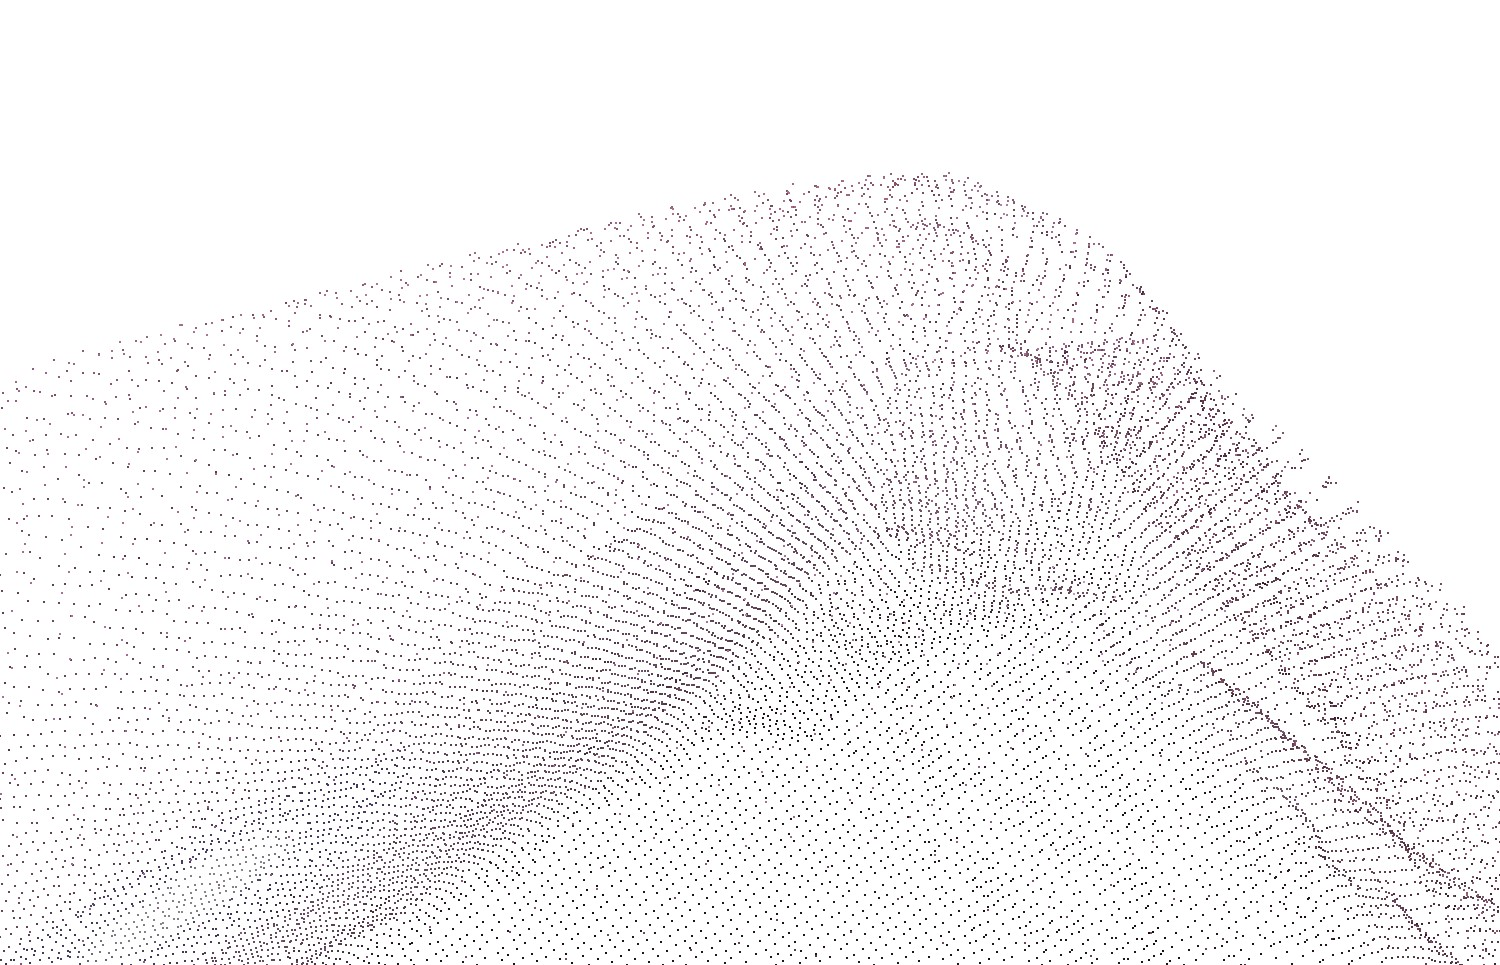
\includegraphics[width=0.95\linewidth]{img/2_grundlagen/points.jpg}
        \centering
        \caption{Ungefilterte Punktwolke}
        \label{img:points}
    \end{subfigure}
    \begin{subfigure}{0.48\textwidth}
        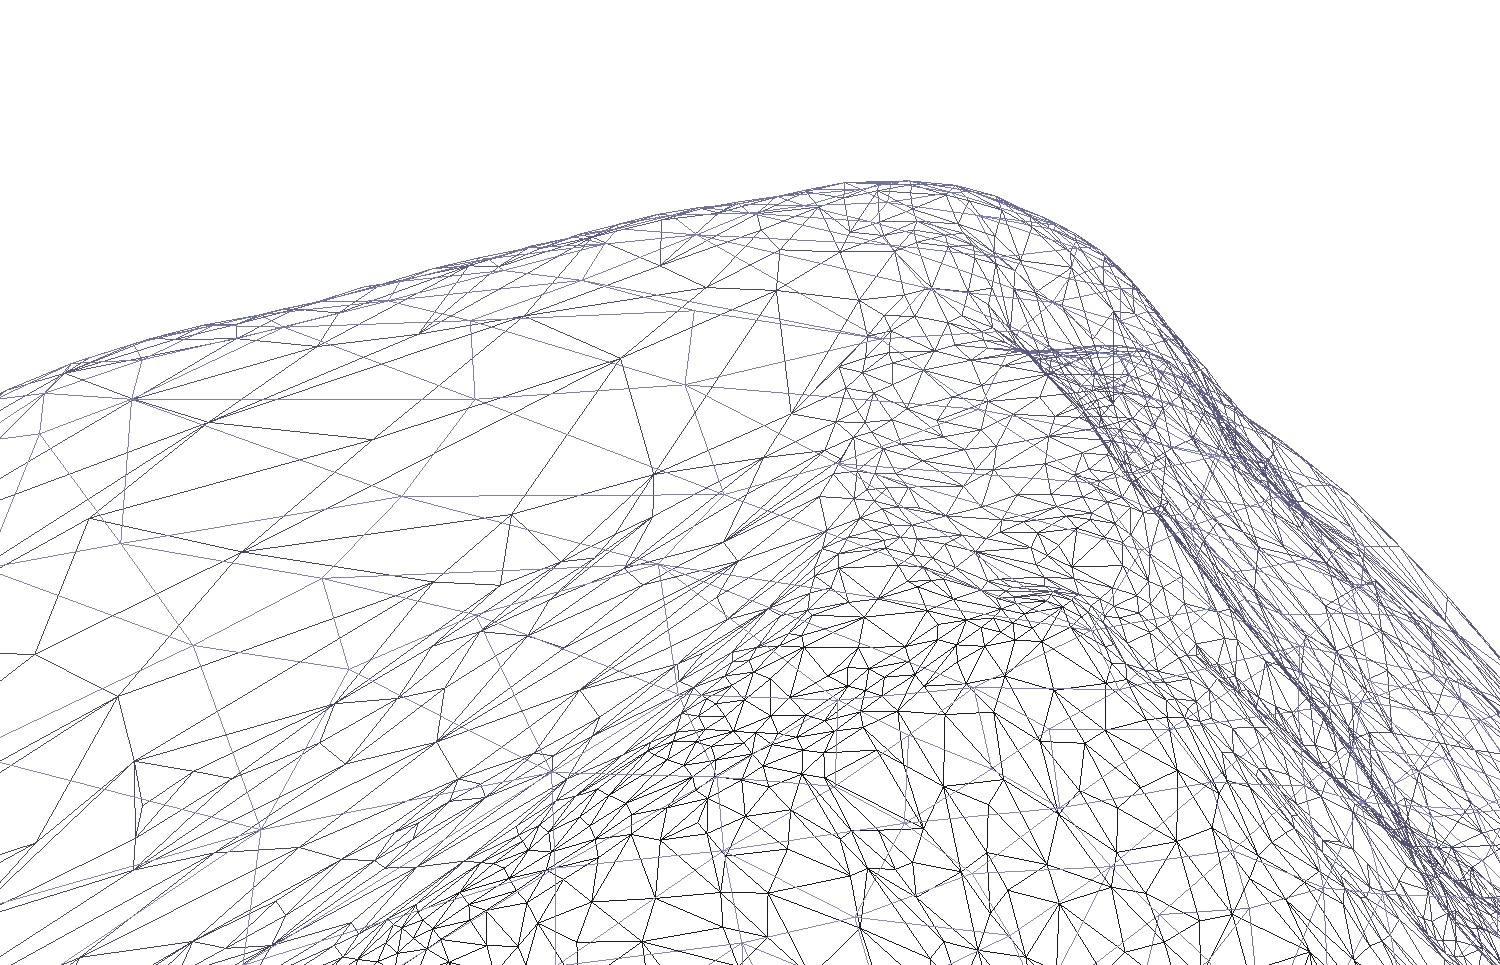
\includegraphics[width=0.95\linewidth]{img/2_grundlagen/mesh.jpg}
        \centering
        \caption{3D-Mesh mit gefilterten Punkten}
        \label{img:mesh}
    \end{subfigure}
    \caption{Vermaschung der Punktwolke}
    \label{img:meshing}
\end{figure}

Die Screened Poisson Surface Reconstruction ist ein Verfahren, das auf der Poisson-Gleichung basiert. Diese Gleichung beschreibt die Beziehung zwischen einer Funktion und ihrer Ableitung. Bei der Screened Poisson Surface Reconstruction wird diese verwendet, um die Oberfläche zu glätten und zu interpolieren. Dabei werden die Punkte in eine Gitterstruktur überführt und die Oberfläche durch die Lösung der Poisson-Gleichung bestimmt. Dieser Ansatz berücksichtigt auch die Ausrichtung der Punkte, um eine genauere Rekonstruktion der Oberfläche zu erzielen. \citep[vgl.][]{spsr}


\section{Texturierung}
Abschließend wird das Modell texturiert. Hierfür werden die Bilder, die zur Erstellung des Modells genutzt wurden, auf das Modell projiziert. Außerdem werden Helligkeits- und Farbunterschiede der Bilder ausgeglichen. \citep[vgl.][S. 54f]{opendronemap}

Vorteil der Texturierung ist, dass das Modell meist realistischer wirkt und fehlende Informationen, beispielsweise fehlende Punkte, überdeckt werden können. Nachteilig ist, dass die Texturierung hierdurch auch Informationen verdeckt. So kann bei einem nur schattierten Modell die Struktur des 3D-Modelles deutlich besser erkannt werden \citep[vgl.][S. 702]{luhmann}. Beispielhaft ist dieses in \autoref{img:texturierung} an dem später auch für die Überprüfungen (siehe \autoref{c:versuche}) verwendeten Testkörper dargestellt. Dieser hat beispielsweise auf der Rückseite (rechts im Bild) einige Einkerbungen, welche im texturierten Modell (siehe \autoref{img:mit_textur}) kaum erkennbar sind. Im ausschließlich schattierten Modell (siehe \autoref{img:ohne_textur}) sind diese hingegen deutlich sichtbar.

\begin{figure}[htbp]
    \centering
    \begin{subfigure}{0.49\textwidth}
        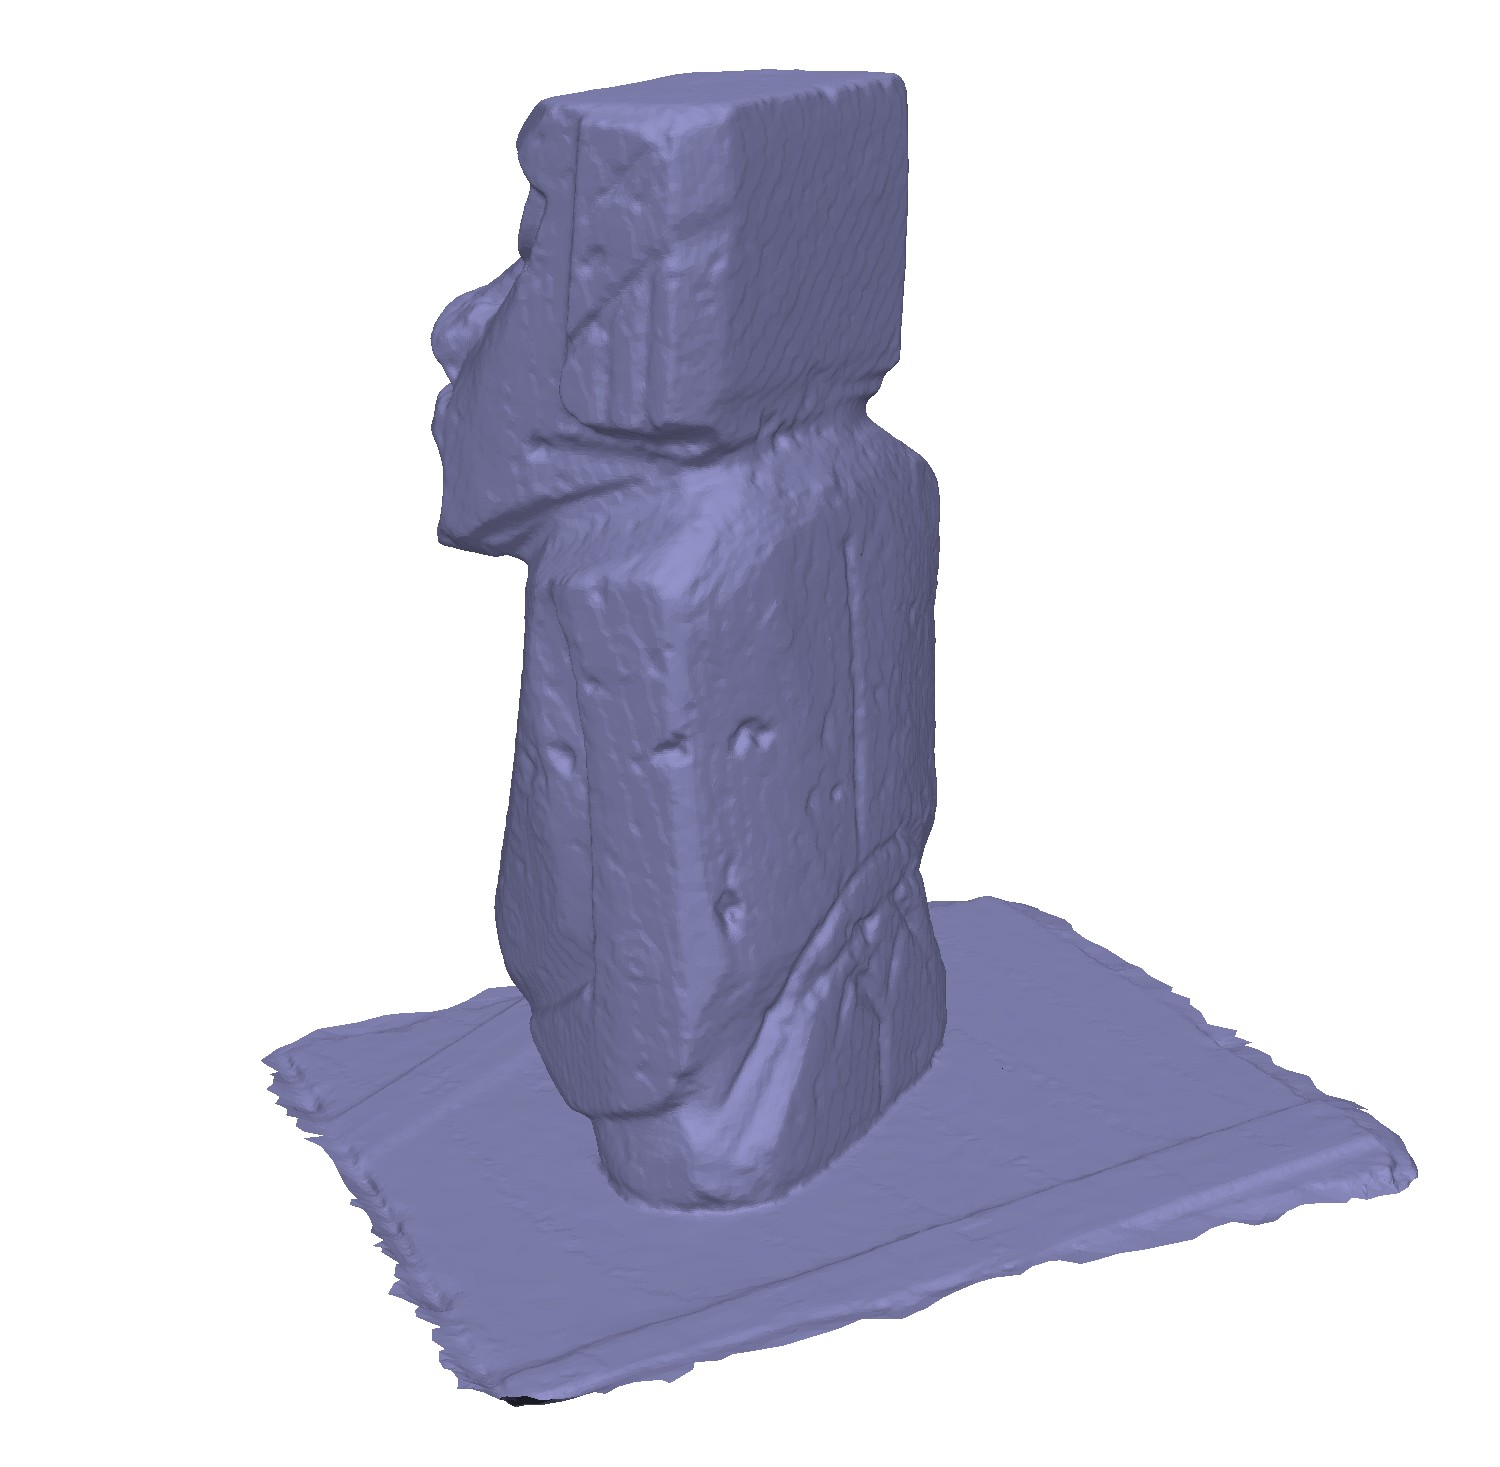
\includegraphics[width=1\linewidth]{img/2_grundlagen/solid.jpg}
        \centering
        \caption{3D-Modell ohne Textur}
        \label{img:ohne_textur}
    \end{subfigure}
    \begin{subfigure}{0.49\textwidth}
        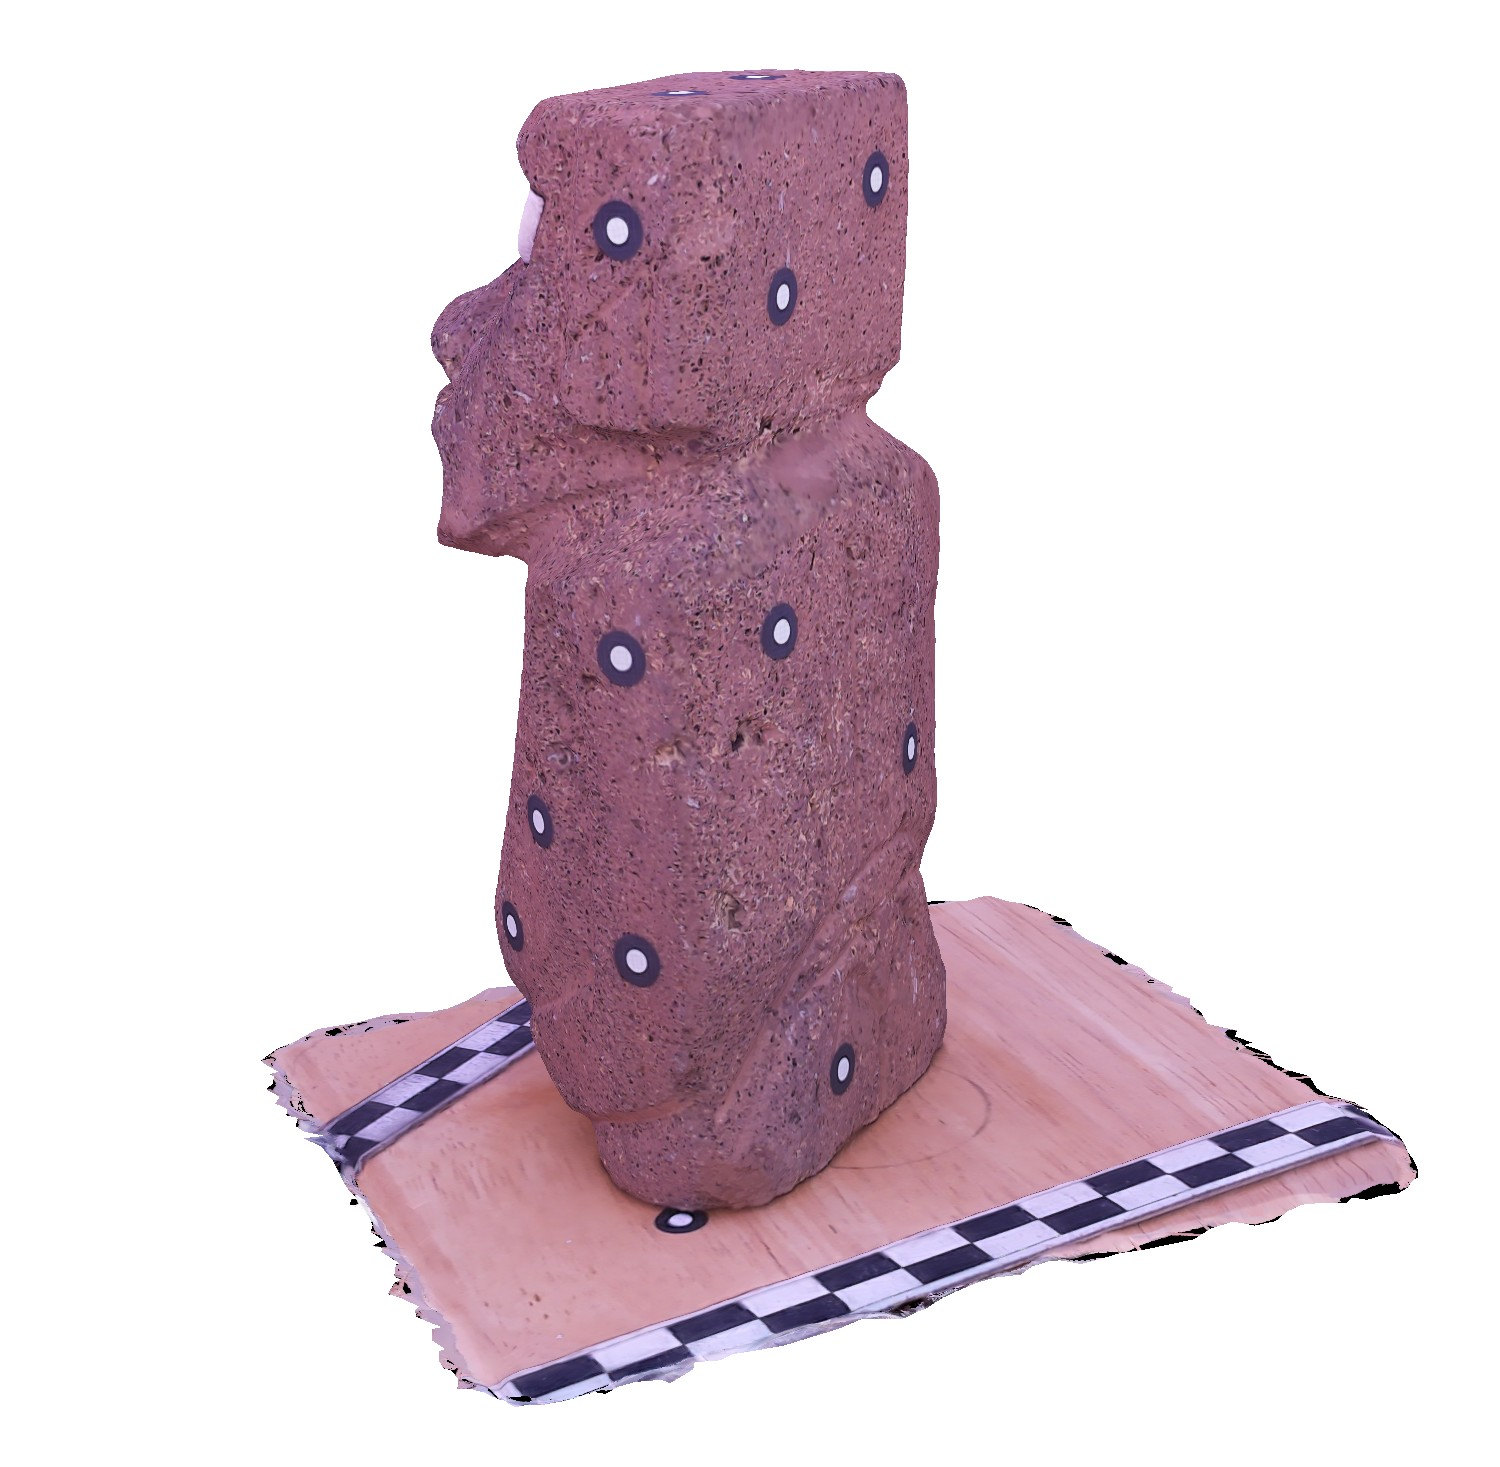
\includegraphics[width=1\linewidth]{img/2_grundlagen/textur.jpg}
        \centering
        \caption{3D-Modell mit Textur}
        \label{img:mit_textur}
    \end{subfigure}
    \caption{3D-Modell ohne und mit Textur}
    \label{img:texturierung}
\end{figure}

\biblio
\end{document}